\documentclass[brazil, a4paper,12pt]{article}
\bibliographystyle{plain}
\usepackage[brazil]{babel}
\usepackage{graphicx}
\usepackage{geometry}
\usepackage[utf8]{inputenc}
\usepackage[T1]{fontenc}
\usepackage{url}
\usepackage{hyperref}
\usepackage{listings}
\usepackage{indentfirst}
\usepackage[usenames]{color}
\geometry{a4paper,left=3cm,right=3cm,top=2.5cm,bottom=2.5cm}

\usepackage[nottoc,notlot,notlof]{tocbibind}%para as referencias aparecer na tableofcontents

\usepackage{listings}
\usepackage{listingsutf8}
\usepackage{xcolor}
\usepackage{upquote}
\usepackage{hyperref}


\begin{document}

\lstdefinestyle{sd}{
	showstringspaces=false,
	language=Python,
	keywordstyle=\color{blue},
	breaklines,
	basicstyle=\ttfamily\small,
	upquote=true,
	showspaces = false,
	morestring=[b]",
	frame=tlrb,
	frame=shadowbox,
	extendedchars=\true,
    inputencoding=utf8/latin1,
    numbers=left,
    moredelim=**[is][\color{blue}]{|}{|},
    literate={á}{{\'a}}1 {ã}{{\~a}}1 {é}{{\'e}}1 {ç}{c}1 {í}{{\'i}}1 {ó}{{\'o}}1 {ú}{{\'u}}1 {õ}{{\~o}}1 {à}{{\`a}}1
}

%\begin{lstlisting}[style=sd]
%\end{lstlisting}

\begin{titlepage}

  \vfill

  \begin{center}
    \begin{large}
      Universidade Federal de Ouro Preto
    \end{large}
  \end{center}

  \begin{center}
    \begin{large}
      Instituto de Ciências Exatas e Aplicadas
    \end{large}
  \end{center}

  \begin{center}
    \begin{large}
      Departamento de Computação e Sistemas
    \end{large}
  \end{center}

  \vfill

  \begin{center}
    \begin{Large}
	      \textbf{Sistemas Distibuídos} \\
	        Relatório do Trabalho Prático I\\
    \end{Large}
  \end{center}


  \vfill

  \begin{center}
    \begin{large}
      Bruno Lacerda Pêgo - 13.2.8300\\ Leonardo de Souza Nogueira - 13.2.8289
    \end{large}
  \end{center}

  \begin{center}
    \begin{large}
      Professor - Theo Lins
    \end{large}
  \end{center}

  \vfill

  \begin{center}
    \begin{large}
      João Monlevade \\
      \today \\
    \end{large}
  \end{center}

\clearpage
\end{titlepage}

\tableofcontents
\newpage

\section{Introduç\~ao}

\subsection{Descriç\~ao do Problema}

\noindent Neste trabalho prático, deve-se implementar\footnote{Este trabalho foi implementado utilizando a linguagem \emph{Python3.4}} a comunicação distribuída de uma Indústria.

	\begin{enumerate}
		\item Clientes:
		\begin{itemize}
			\item Responsável por solicitar os produtos a Indústria.
		\end{itemize}
		
		\item Fornecedores:
		\begin{itemize}
			\item Responsável por fornecer matéria prima.
		\end{itemize}
		
		\item Controlador de Produção (Multithread):
		\begin{itemize}
			\item Responsável por gerenciar a produção, receber solicitações dos clientes, verificar
matéria prima.
		\end{itemize}
		
		\item Linhas de Produções:
		\begin{itemize}
			\item Equipamento de Produção: Responsável por transformar a matéria prima em
produto final.
			\item Sensor Inicial: Verifica os produtos que entraram na linha de produção.
			\item Sensor Final: Verifica se o produto ficou correto.
		\end{itemize}
	\end{enumerate}
	
\subsection{Vis\~ao geral sobre o funcionamento do programa}

No trabalho temos basicamente quatro módulos onde cada um se relaciona com um ou mais módulos do sistema se necessário.

No nosso caso, o Cliente relaciona com o Controlador de Produção onde ele pode solicitar a produção de cadeiras\footnote{A indústria implementada no trabalho produz cadeiras}.

O Controlador se comunica com o cliente, solicita matéria prima para o fornecedor e envia os produtos para produção na Linha de Produção. 

O Fornecedor comunica com o Controlador de Produção, enviando quando necessário a matéria prima solicitada.

A Linha de Produção tem como função produzir o produto solicitado pelo Controlador de Produção, a capacidade da linha de produção é de 30 cadeiras no máximo por produção, caso haja falha na produção a mesma deve informar ao Controlador, que deve enviar novamente para a Linha de Produção nova matéria prima para que o total de produtos perfeitos solicitados pelo cliente sejam produzidos.

\newpage

\section{Implementaç\~ao}

No trabalho não foi utilizada alguma estrutura de dados em específico. Durante a execução, pode-se deparar com \emph{"MP"} que significa \emph{matéria prima}.

\begin{enumerate}

\item Cliente:

\begin{itemize}

\item Método \emph{main} (os comentários apresentam informações suficiente):

\begin{lstlisting}[style=sd]
#Método principal onde se chama o construtor do cliente
def main():
    print("Fábrica")
    cli = cliente()

    #Laço em que o usuário terá a opção de escolher se deseja fazer um pedido
    while True:
        resp = input("Deseja fazer um pedido [s/n]? ")

        #Se o usuário digita 's' ou 'S' então ele digita uma quantidade de produtos para fazer
        if resp.lower() == 's':
            resp = input("Quantos cadeiras voce deseja que sejam produzidas? ")
            cli.pedido(resp)

        # Se o usuário digita 'n' ou 'N' então ele sai da aplicação e a conexão é fechada
        # Caso o primeiro comando seja 'n' ou 'N', não houve criação do socket, logo deve-se tratar
        # e sair sem tentar fechar socket
        elif resp.lower() == 'n':
            try:
                cli.s.close()
            except Exception:
                pass
            break

\end{lstlisting}

\item Método \emph{pedido} (os comentários apresentam informações suficiente):

\begin{lstlisting}[style=sd]
#Método onde se cria um socket para comunicação com o controlador de produção
    def pedido(self, resp, v = None):

        #O bloco abaixo cria o socket, conecta ao controlador e envia a quantidade de produtos que o usuário digitou
        self.s = socket.socket()
        self.s.connect((self.hostconnectControlador, self.port))
        self.s.send(resp.encode('utf-8'))
        #A linha abaixo fica esperando a resposta do controlador e logo após fecha o socket de comunicação
        msg = self.s.recv(128).decode('utf-8')
        print("Resposta do Controlador de Produção: " + msg)
        self.s.close()


\end{lstlisting}

\end{itemize}

\item Controlador de Produção:

\begin{itemize}

\item Método \emph{tratarPedido} (os comentários apresentam informações suficiente):

\begin{lstlisting}[style=sd]
# Abaixo o método de tratar pedido recebido pelo cliente e direcionar se precisa de mais matéria prima
    # se precisa de reenviar para linha de produção matéria prima para produção de outro produto (substituir defeituoso)
    def tratarPedido(self, cliente, endr):
        global estoque
        print("Tem " + str(estoque) + " unidades de MP em estoque.")

        # Abaixo Fica à espera de uma mensagem do cliente, se a msg não conter nada então fecha a conexão
        msg = cliente.recv(128).decode('utf-8')
        if not msg:
            cliente.close()
        print("Cliente: " + str(endr), "-> Produção solicitada: " + msg + " Cadeiras.")


        # Abaixo é feita a converão da msg recebida em um número INT
        qtd_solicitada = int(msg)

        # Se o tanto de matéria prima para fazer um produto for menor que a quantidade solicitada pelo cliente
        # então é chamada a função de solicitar mais matérias primas ao fornecedor, logo após é feita a subtração
        # no estoque a quantidade referente a solicitação do cliente
        if(estoque < qtd_solicitada):
            print(str(estoque) + " unidades de MP em estoque...")
            print("Solicitando matéria prima...")
            self.solicitarMateriaPrima(str(qtd_solicitada - estoque))
            print("Matéria prima recebida...")
        estoque -= qtd_solicitada

        # A linha de producao tem uma capacidade que é definida pela variável "capacidade_linhaProducao"
        # que é solicitado a cada iteração do laço e caso necessário é feito no final uma solicitação do restante
        # Abaixo também é medido o tempo gasto pela linha de produção para fazer os produtos
        tempo_inicial = time.time()
        while qtd_solicitada != qtd_solicitada % self.capacidade_linhaProducao:
            print("Em produção: " + str(self.capacidade_linhaProducao))
            self.enviarParaProducao(str(self.capacidade_linhaProducao))
            qtd_solicitada -= self.capacidade_linhaProducao

        if(qtd_solicitada > 0):
            print("Em produção: " + str(qtd_solicitada))
            self.enviarParaProducao(qtd_solicitada)
        print("O tempo de produção foi: %s segundos" %(time.time() - tempo_inicial))

        # Como todos produtos já estão prontos agora é só chamar o método de enviar a resposta para o cliente
        print("Todos os produtos solicitados estão prontos!")
        print("Estoque atual: " + str(estoque) + " unidades de MP em estoque.")
        self.enviarPedidoParaCliente(cliente)

        # Agora a conexão pode ser fechada
        cliente.close()


\end{lstlisting}

\item Método \emph{solicitarMateriaPrima}:

Assim como nos métodos anteriores, nessa função é criado um \emph{socket} que comunica com o módulo Fornecedor

\begin{lstlisting}[style=sd]
# Método de solicitar matéria prima ao fornecedor
    def solicitarMateriaPrima(self, qtd):

        qtd = str(qtd)

        # Usa-se a variável de estoque global que receberá a matéria prima do fornecedor
        global estoque
        sm = socket.socket()
        sm.connect((self.hostFornecedor, self.porta_fornecedor))
        sm.send(qtd.encode('utf-8'))
        materia_prima_recebida = sm.recv(128).decode('utf-8')
        estoque += int(materia_prima_recebida)
        sm.close()
        return 0

\end{lstlisting}

\item Método \emph{enviarParaProducao} (os comentários apresentam informações suficiente):

\begin{lstlisting}[style=sd]
# Método que envia para a linha de produção a matéria prima (nesse caso quantidade de matéria prima)
    def enviarParaProducao(self, qtd):

        qtd = str(qtd)
        # Usa-se a variável referente ao estoque para controle ao retirar materias primas dele
        global estoque

        #é criado então um socket para tais transações
        lp = socket.socket()
        lp.connect((self.hostLinhaProducao, self.porta_linhaProducao))
        lp.send(qtd.encode('utf-8'))

        # A resposta é a quantidade de materiais com defeito que deverão ser reenviados para a Linha de Produção
        resposta = lp.recv(128).decode('utf-8')

        # Enquanto a resposta é diferente de zero significa que há necessidade de pegar matéria prima no
        # estoque e enviar a linha de produção para repor os produtos defeituosos. Caso contrário significa
        # que não houve perda de produtos ou defeitos na linha de produção, então fecha a conexão
        while resposta != '0':

            if(estoque < int(resposta)):
                print("Houve um erro na produção...")
                print("Estoque insuficiente - Solicitando materiais...")
                self.solicitarMateriaPrima(resposta)
                lp.send(resposta.encode('utf-8'))
                estoque -= int(resposta)
            else:
                print("Houve um erro na produção...")
                lp.send(resposta.encode('utf-8'))
                estoque -= int(resposta)

            resposta = lp.recv(128).decode('utf-8')

        print("Produção concluída!")
        lp.close()

\end{lstlisting}

\end{itemize}

\item Fornecedor:

\begin{itemize}

\item Método \emph{enviarParaProducao} (os comentários apresentam informações suficiente):

\begin{lstlisting}[style=sd]
# Método que recebe a quantidade de matéria prima deve ser enviada e as retornam
    def fornecerMateriaPrima(self, cliente, endr):
        msg = cliente.recv(128).decode('utf-8')
        qtd_solicitada = int(msg)
        print(msg + " unidades de MP solicitadas...")
        print("Enviando " + str(qtd_solicitada) + " unidades de MP.")
        cliente.send(str(qtd_solicitada).encode('utf-8'))
        cliente.close()

\end{lstlisting}

\end{itemize}

\item Linha de Produção:

\begin{itemize}

\item Método \emph{enviarParaProducao} (os comentários apresentam informações suficiente):

\begin{lstlisting}[style=sd]
# Método que fará o produto (recebe a quantidade de produto que deve ser feito)
    def produz(self, qtd):
        nqtd = int(qtd)

        # Inicialmente define uma váriavel i como contador para o laço e outra
        # que vai contar o número de produtos defeituosos
        # o laço trata em cada if se o produto está defeituoso e caso sim adiciona +1 em produtosComDefeitos
        # Faz um produto de cada vez
        i = 0
        produtosComDefeitos = 0
        while i < nqtd:
            if self.sensorInicial() == True:
                if self.equipamentoDeProducao() == True:
                    if self.sensorFinal() == True:
                        print("Produto produzido: ", i+1)
                    else:
                        produtosComDefeitos += 1
                else:
                    produtosComDefeitos += 1
            else:
                produtosComDefeitos += 1

            i += 1
        # Finalmente retorna o resultado de produtos com defeito e a quantidade produzida independente do defeito
        self.retornaResultado(produtosComDefeitos, nqtd)

\end{lstlisting}

\item Métodos \emph{sensores}:

Os métodos abaixo define a quantide de erro que pode ocorrer na produção das cadeiras, e pode ter uma taxa de defeito é 10\% em cada sensor.

\begin{lstlisting}[style=sd]
# Método que "verifica" se a matéria prima está ou não com defeito (apenas gera um número aleatório)
    def sensorInicial(self):
        defeito = randrange(0, 10)
        if defeito == 1:
            return False
        return True

    # Método que "verifica" o produto durante o processo de produção (apenas gera um número aleatório)
    def equipamentoDeProducao(self):
        defeito = randrange(0, 10)
        if defeito == 2:
            return False
        return True

    # Método que "verifica" o produto final (apenas gera um número aleatório)
    def sensorFinal(self):
        defeito = randrange(0, 10)
        if defeito == 2:
            return False
        return True
        
\end{lstlisting}

\end{itemize}

\end{enumerate}


\section{Listagem de testes executados}

\begin{enumerate}

\vfill

\item Teste 1:

Neste primeiro teste foi solicitado para produzir 20 cadeiras, como pode-se observar pelas imagens houve cadeiras produzidas com defeito, no caso 5 cadeiras defeituosas e com isso foi solicitado novamente a produção de mais 5 cadeiras.

\begin{figure}[h]
\centering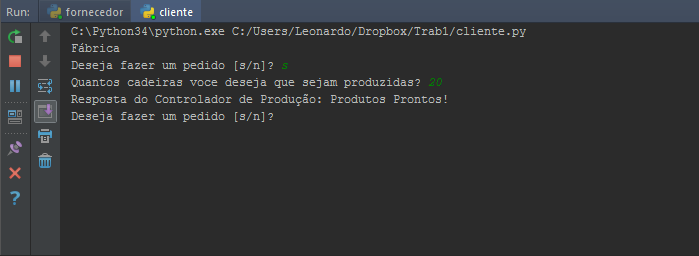
\includegraphics[width=90mm,scale=0.5]{testes/cliente1.png}
\caption{Execuç\~ao do Cliente}
\label{fig:cliente1}
\end{figure}

\begin{figure}[h]
\centering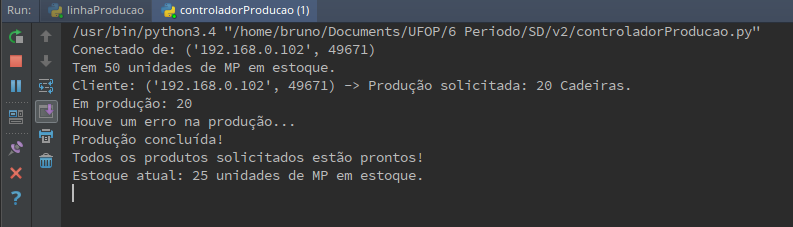
\includegraphics[width=90mm,scale=0.5]{testes/controlador1.png}
\caption{Execuç\~ao do Controlador de Produç\~ao}
\label{fig:controlador1}
\end{figure}

\begin{figure}[h]
\centering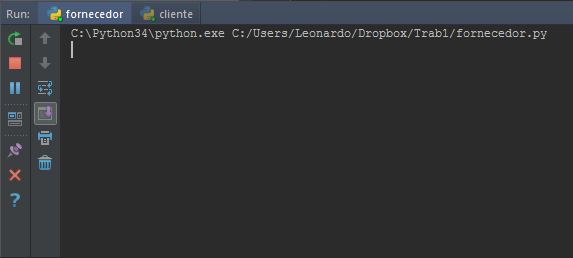
\includegraphics[width=90mm,scale=0.5]{testes/fornecedor1.png}
\caption{Execuç\~ao do Fornecedor}
\label{fig:fornecedor1}
\end{figure}

\begin{figure}[h]
\centering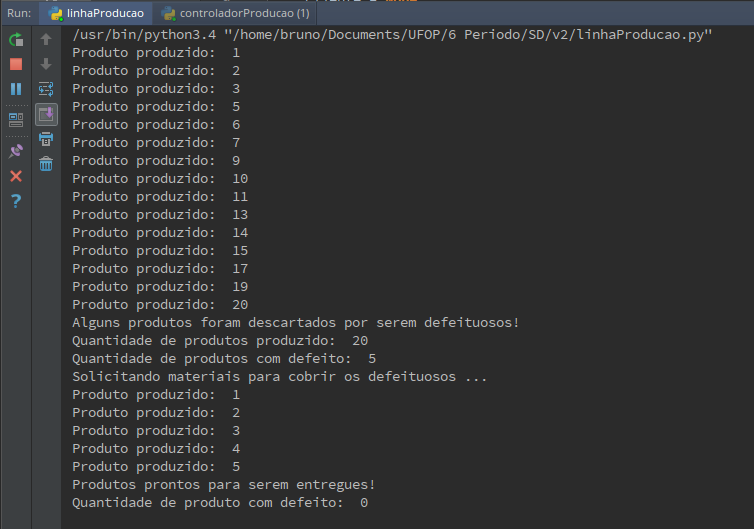
\includegraphics[width=90mm,scale=0.5]{testes/linhaproducao1.png}
\caption{Execuç\~ao da Linha de Produç\~ao}
\label{fig:linhaproducao1}
\end{figure}

\vfill
\clearpage

%\newpage

\vfill

\item Teste 2:

Neste segundo teste foi solicitado para produzir 68 cadeiras, como a linha de produção só produz 30 cadeiras por vez é necessário que o controlador mantenha controle para que haja a produção total das cadeiras solicitadas, pode-se observar pelas imagens que houve cadeiras produzidas com defeito, sempre quando há defeito o controlador solicita novamente que mais cadeiras seja contruidas para atender a solicitação do cliente.

\begin{figure}[h]
\centering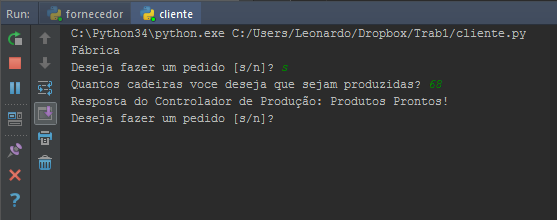
\includegraphics[width=90mm,scale=0.5]{testes/cliente2.png}
\caption{Execuç\~ao do Cliente}
\label{fig:cliente2}
\end{figure}

\begin{figure}[h]
\centering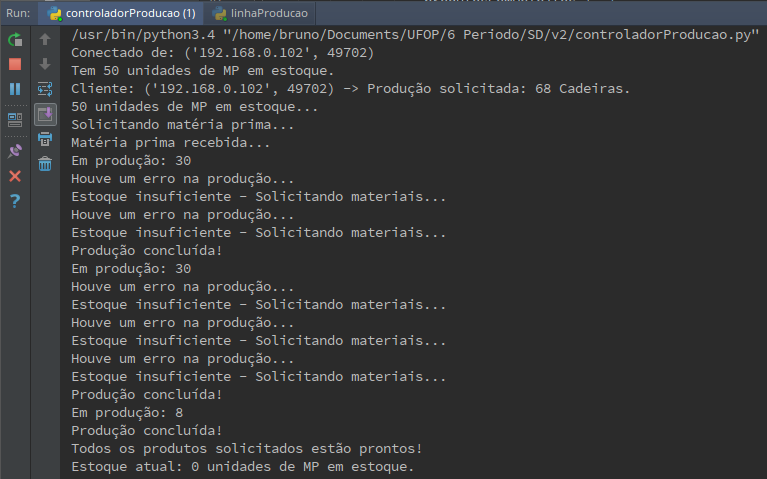
\includegraphics[width=90mm,scale=0.5]{testes/controlador2.png}
\caption{Execuç\~ao do Controlador de Produç\~ao}
\label{fig:controlador2}
\end{figure}

\begin{figure}[h]
\centering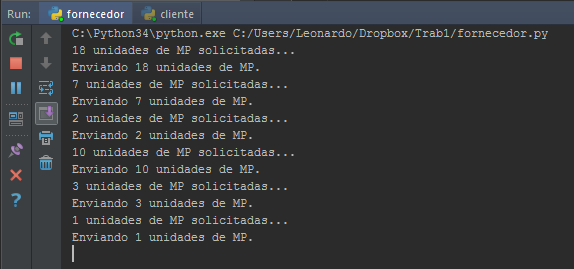
\includegraphics[width=90mm,scale=0.5]{testes/fornecedor2.png}
\caption{Execuç\~ao do Fornecedor}
\label{fig:fornecedor2}
\end{figure}

\begin{figure}[h]
\centering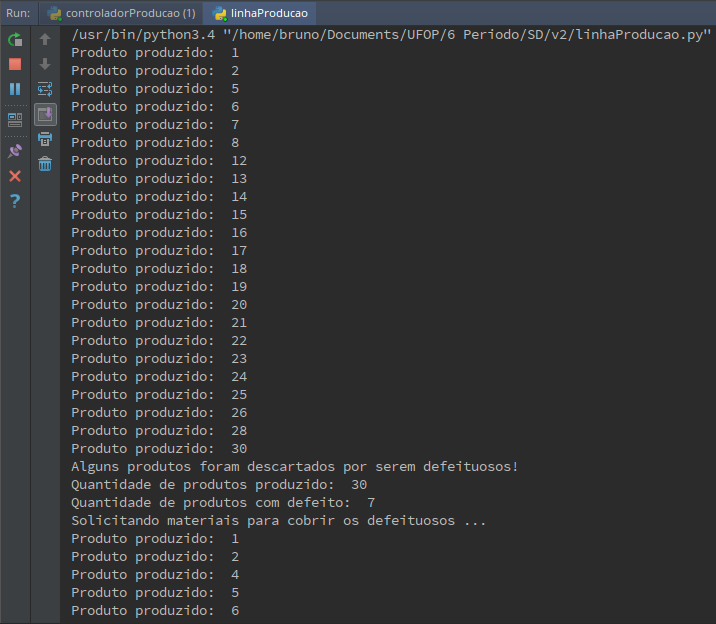
\includegraphics[width=90mm,scale=0.5]{testes/linhaProducao2_1.png}
\caption{Execuç\~ao da Linha de Produç\~ao (1)}
\label{fig:linhaproducao2}
\end{figure}

\begin{figure}[h]
\centering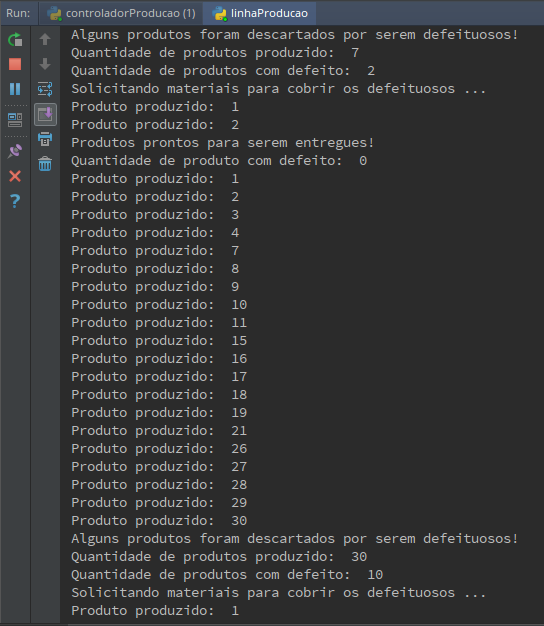
\includegraphics[width=90mm,scale=0.5]{testes/linhaProducao2_2.png}
\caption{Execuç\~ao da Linha de Produç\~ao (2)}
\label{fig:linhaproducao2}
\end{figure}

\begin{figure}[h]
\centering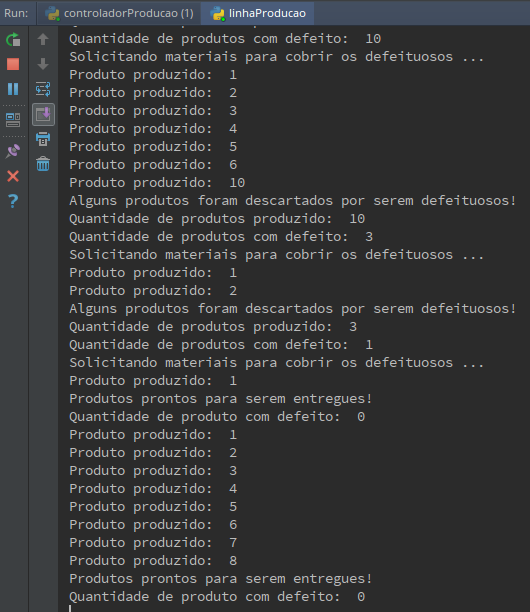
\includegraphics[width=90mm,scale=0.5]{testes/linhaProducao2_3.png}
\caption{Execuç\~ao da Linha de Produç\~ao (3)}
\label{fig:linhaproducao2}
\end{figure}

\vfill
\clearpage

\end{enumerate}

\newpage

\section{Conclus\~ao}
A implementação do trabalho na linguagem de programação Python não foi muito complicada devido esta oferecer uma grande simplicidade de implementação. Contudo, houve um trabalho a mais para conseguir desenvolver a comunicação entre os módulos do sistema de modo que ficassem sincronizados e coerentes.

\nocite{*}
	\bibliography{relatorioTPI}
  	\bibliographystyle{abbrv}


\end{document}